% 第4章第4节：平滑逼近（磨光与导数交换、整域光滑逼近、边界延拓与Lipschitz区域）。

\section{平滑逼近}
\label{sec:sob-smoothing}

Sobolev函数可以有尖点、可以无界，直接对它做计算常常不方便。一个反复使用的策略是：先对光滑函数证明某个估计，再用光滑函数逼近一般的Sobolev函数，让估计在极限中保留下来。这要求光滑函数在Sobolev范数下稠密，而“稠密”还要说清楚是哪一类光滑函数。本节分三个层次讨论：在区域内部做局部平均，并让平均与弱导数交换；把局部结果拼成整个区域上的逼近；再借边界延拓得到光滑到边界的逼近。三种要求一个比一个强，不能笼统地说“平滑一下”就同时满足。

\subsection{局部平滑与导数交换}
\label{sec:sob-mollification}

把一个函数在每一点附近作加权平均，平均的权重若是光滑的，结果便是光滑函数；平均的范围越小，结果越接近原函数。第~\ref{sec:sob-test-functions}节的归一化凸起$\rho_\varepsilon$（式~\eqref{eq:sob-mollifier}）正好可以充当权重。

\paragraph{磨光的定义}
设$u\in L^1_{\mathrm{loc}}(\Omega)$。为了保证平均只读取$\Omega$内的值，记
\[
 \Omega_\varepsilon=\{x\in\Omega:\operatorname{dist}(x,\partial\Omega)>\varepsilon\}
\]
（$\Omega=\mathbb R^d$时$\Omega_\varepsilon=\mathbb R^d$）。对$x\in\Omega_\varepsilon$，球$\overline B(x,\varepsilon)$落在$\Omega$内，定义
\begin{equation}
 u_\varepsilon(x)=(u*\rho_\varepsilon)(x)=\int_\Omega u(y)\,\rho_\varepsilon(x-y)\,\mathrm dy=\int_{|z|\le\varepsilon}u(x-z)\,\rho_\varepsilon(z)\,\mathrm dz ,
 \label{eq:sob-mollification}
\end{equation}
称为$u$的\term{磨光}（mollification），$\rho_\varepsilon$称为\term{磨光核}（mollifier）。积分号$*$即卷积，这里只用到它作为加权平均的含义。由于$\rho_\varepsilon\ge0$、$\int\rho_\varepsilon=1$，$u_\varepsilon(x)$是$u$在球$B(x,\varepsilon)$上的加权平均，权重集中在中心附近。

磨光后的函数是光滑的。对$x$在$\Omega_\varepsilon$的紧子集$K'$上变化，被积函数$u(y)\rho_\varepsilon(x-y)$的各阶$x$导数$u(y)D^\alpha\rho_\varepsilon(x-y)$被$\sup|D^\alpha\rho_\varepsilon|\cdot|u(y)|\mathbf 1_{K''}(y)$控制，其中$K''=\{y:\operatorname{dist}(y,K')\le\varepsilon\}$是$\Omega$内的紧集，控制函数可积。按第~\ref{sec:multivariable-parameter-integrals}节可以在积分号下求导，所以$u_\varepsilon\in C^\infty(\Omega_\varepsilon)$，并且
\begin{equation}
 D^\alpha u_\varepsilon(x)=\int_\Omega u(y)\,(D^\alpha\rho_\varepsilon)(x-y)\,\mathrm dy .
 \label{eq:sob-mollifier-derivative}
\end{equation}
图~\ref{fig:sob-mollifier}(a)画出一维的$\rho_\varepsilon$：$\varepsilon$减半，支撑减半，高度加倍，面积保持为$1$。

\begin{figure*}[!htb]
  \centering
  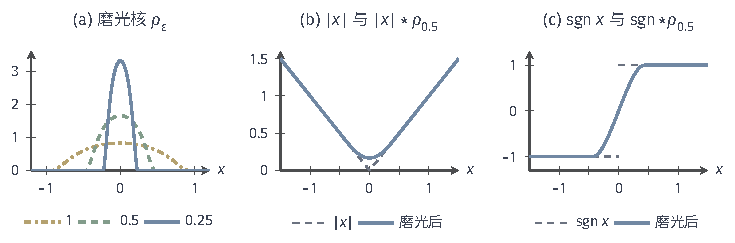
\includegraphics[width=124.4mm]{figures/02-abstract-mathematics/03-function-spaces/tikz/c4-mollifier/figure.pdf}
  \caption{一维磨光。(a)~磨光核$\rho_\varepsilon$，$\varepsilon=1,0.5,0.25$：支撑为$[-\varepsilon,\varepsilon]$，峰值约$0.829/\varepsilon$，面积均为$1$。(b)~$|x|$（虚线）与$|x|*\rho_{0.5}$（实线）：尖点被抹平，原点值约$0.167$，在$|x|\ge0.5$处两者重合。(c)~$\operatorname{sgn}x$与$\operatorname{sgn}*\rho_{0.5}$：后者光滑地从$-1$升到$1$，它恰好是(b)中光滑曲线的导数，体现$(|x|*\rho_\varepsilon)'=\operatorname{sgn}*\rho_\varepsilon$。}
  \label{fig:sob-mollifier}
\end{figure*}

\paragraph{$L^p$中的恢复}
要让磨光成为逼近，需要说明$u_\varepsilon\to u$。我们先考虑$\Omega=\mathbb R^d$且$u\in L^p(\mathbb R^d)$，$1\le p<\infty$；一般区域的情形随后用截断归结到这里。证明分三步。

第一步，磨光不放大$L^p$范数。$\rho_\varepsilon(x-\cdot)\,\mathrm dy$是质量为$1$的测度，对它使用Hölder不等式（$p>1$时把被积函数写成$|u|\rho_\varepsilon^{1/p}\cdot\rho_\varepsilon^{1/q}$），得
\[
 |u_\varepsilon(x)|^p\le\int|u(y)|^p\rho_\varepsilon(x-y)\,\mathrm dy .
\]
两边对$x$积分，非负被积函数可交换积分次序（定理~\ref{thm:analysis-tonelli-fubini}），而$\int\rho_\varepsilon(x-y)\,\mathrm dx=1$，于是
\begin{equation}
 \|u_\varepsilon\|_{L^p}\le\|u\|_{L^p} .
 \label{eq:sob-mollifier-contraction}
\end{equation}
同样的论证用于平均值之差，给出
\begin{equation}
 \|u_\varepsilon-u\|_{L^p}\le\sup_{|z|\le\varepsilon}\|u(\cdot-z)-u\|_{L^p} ,
 \label{eq:sob-mollifier-translation}
\end{equation}
因为$u_\varepsilon(x)-u(x)=\int[u(x-z)-u(x)]\rho_\varepsilon(z)\,\mathrm dz$也是关于质量为$1$的测度的平均。于是问题化为平移的连续性：小平移是否只引起小的$L^p$误差。

第二步，对紧支撑连续函数证明平移连续性。设$g$连续且支撑在紧集$K_0$内。由Heine--Cantor定理（定理~\ref{thm:metric-heine-cantor}），$g$一致连续，所以$\sup_x|g(x-z)-g(x)|\to0$（$z\to0$）。$|z|\le1$时差函数支撑在$\{x:\operatorname{dist}(x,K_0)\le1\}$内，这个集合的测度有限，记为$M$，于是$\|g(\cdot-z)-g\|_{L^p}\le M^{1/p}\sup_x|g(x-z)-g(x)|\to0$。

第三步，推广到一般$L^p$。由第~\ref{sec:fs-density-separability}节，紧支撑连续函数在$L^p(\mathbb R^d)$中稠密（$1\le p<\infty$）：先用简单函数逼近，再用连续截断逼近有限测度集合的示性函数。任给$\eta>0$，取这样的$g$使$\|u-g\|_{L^p}<\eta$。平移不改变$L^p$范数，所以
\[
 \begin{aligned}
 \|u(\cdot-z)-u\|_{L^p}&\le\|u(\cdot-z)-g(\cdot-z)\|_{L^p}+\|g(\cdot-z)-g\|_{L^p}+\|g-u\|_{L^p}\\
 &<2\eta+\|g(\cdot-z)-g\|_{L^p} .
 \end{aligned}
\]
令$z\to0$，右端的上极限不超过$2\eta$，而$\eta$任意，故平移连续性成立。代回式~\eqref{eq:sob-mollifier-translation}，得到$\|u_\varepsilon-u\|_{L^p}\to0$。

对一般开集$\Omega$和$u\in L^p(\Omega)$，取开集$V$，其闭包是$\Omega$内的紧集，记$\delta=\operatorname{dist}(V,\partial\Omega)$。把$u$在$\Omega$外补成零得到$\tilde u\in L^p(\mathbb R^d)$；当$\varepsilon<\delta$时，在$V$上$u_\varepsilon=\tilde u*\rho_\varepsilon$，所以$\|u_\varepsilon-u\|_{L^p(V)}\le\|\tilde u*\rho_\varepsilon-\tilde u\|_{L^p(\mathbb R^d)}\to0$。这就是磨光的局部$L^p$恢复。

$p=\infty$时结论不成立。在$(-1,1)$上，$H_\varepsilon=H*\rho_\varepsilon$连续，而$H$在原点两侧分别为$0$和$1$，所以在原点附近总有一侧满足$|H_\varepsilon-H|\ge1/2$，$\|H_\varepsilon-H\|_{L^\infty}$不趋于零。连续函数的一致极限仍连续，不连续的$L^\infty$函数不可能被连续函数一致逼近。

\paragraph{磨光与弱导数交换}
现在设$u$有弱导数$D^\alpha u\in L^1_{\mathrm{loc}}(\Omega)$。对$x\in\Omega_\varepsilon$，函数$y\mapsto\rho_\varepsilon(x-y)$是$\Omega$上的测试，其$y$导数满足$D_y^\alpha[\rho_\varepsilon(x-y)]=(-1)^{|\alpha|}(D^\alpha\rho_\varepsilon)(x-y)$。从式~\eqref{eq:sob-mollifier-derivative}出发，
\[
 D^\alpha u_\varepsilon(x)=(-1)^{|\alpha|}\int_\Omega u(y)\,D_y^\alpha[\rho_\varepsilon(x-y)]\,\mathrm dy
 =\int_\Omega D^\alpha u(y)\,\rho_\varepsilon(x-y)\,\mathrm dy ,
\]
第二个等号是弱导数的定义~\eqref{eq:sob-weak-derivative}用于这个测试。于是
\begin{equation}
 D^\alpha(u*\rho_\varepsilon)=(D^\alpha u)*\rho_\varepsilon\qquad\text{在 }\Omega_\varepsilon\text{ 上成立}.
 \label{eq:sob-mollifier-commute}
\end{equation}
左端是光滑函数的经典导数，右端是弱导数的磨光。图~\ref{fig:sob-mollifier}(b)(c)在$|x|$上验证了这一点：磨光后的$|x|$的经典导数，正是$\operatorname{sgn}x$的磨光。

把式~\eqref{eq:sob-mollifier-commute}与$L^p$恢复结合，就得到局部的光滑逼近。

\begin{theorem}[局部光滑逼近]
\label{thm:sob-local-approximation}
设$1\le p<\infty$，$u\in W^{k,p}(\Omega)$，$V$为开集且闭包是$\Omega$内的紧集。则$u_\varepsilon\in C^\infty(\Omega_\varepsilon)$，并且当$\varepsilon\to0$时$\|u_\varepsilon-u\|_{W^{k,p}(V)}\to0$。若$\Omega=\mathbb R^d$，则$\|u_\varepsilon-u\|_{W^{k,p}(\mathbb R^d)}\to0$。
\end{theorem}

\begin{proof}
光滑性已在前面证明。对每个$|\alpha|\le k$，由式~\eqref{eq:sob-mollifier-commute}，$D^\alpha u_\varepsilon-D^\alpha u=(D^\alpha u)_\varepsilon-D^\alpha u$在$V$上成立（$\varepsilon<\operatorname{dist}(V,\partial\Omega)$），而$D^\alpha u\in L^p(\Omega)$，由局部$L^p$恢复，它在$L^p(V)$中趋于零。有限多个分量都趋于零，Sobolev范数也趋于零。$\Omega=\mathbb R^d$时用全空间的恢复即可。
\end{proof}

这个定理是连接弱运算与经典计算的桥梁：凡是对光滑函数成立、又只涉及$W^{k,p}$范数连续量的等式或不等式，都可以先对$u_\varepsilon$证明，再令$\varepsilon\to0$。它对$W^{k,\infty}$不成立。例如任何$C^1$函数$v$在$(-1,1)$上都满足$\|v'-\operatorname{sgn}\|_{L^\infty}\ge1$：$v'$在原点连续，在原点附近的右侧与左侧分别接近同一个数$v'(0)$，而$\max(|v'(0)-1|,|v'(0)+1|)\ge1$。所以$|x|$不能在$W^{1,\infty}$范数下被$C^1$函数逼近。

\subsection{整域逼近与边界延拓}
\label{sec:sob-global-approximation}

定理~\ref{thm:sob-local-approximation}只在离边界有正距离的区域上逼近。靠近边界的地方，磨光半径必须越来越小，否则会读到区域外的值。解决办法是把函数切成许多块，每块离边界的距离不同，各自选择合适的磨光半径，再拼回去。切块需要一组光滑的权重。

\paragraph{局部有限的单位分解}
取递增的开集$G_j=\{x\in\Omega:|x|<j,\ \operatorname{dist}(x,\partial\Omega)>1/j\}$，$j\ge1$，并令$G_0=G_{-1}=\varnothing$。每个$G_j$的闭包是$\Omega$内的紧集，$\bigcup_jG_j=\Omega$。令
\[
 V_j=G_{j+1}\setminus\overline{G_{j-1}},\qquad j\ge1 .
\]
这些开集覆盖$\Omega$，并且是\term{局部有限}（locally finite）的：每个$x\in\Omega$属于某个$G_m$，而$G_m$只与$V_1,\ldots,V_{m+1}$相交，所以$x$的邻域$G_m$只与有限多个$V_j$相交。可以证明存在函数$\zeta_j\in C_c^\infty(V_j)$，满足$0\le\zeta_j\le1$，并且
\[
 \sum_{j\ge1}\zeta_j(x)=1\qquad(x\in\Omega).
\]
构造方法是：用引理~\ref{lem:sob-cutoff}在紧集$\overline{G_j}\setminus G_{j-1}$上取等于$1$、支撑在$V_j$内的截断$\eta_j$，则$\sum_i\eta_i$在每点是有限和且处处为正，令$\zeta_j=\eta_j/\sum_i\eta_i$。称$\{\zeta_j\}$为从属于覆盖$\{V_j\}$的\term{单位分解}（partition of unity）。

图~\ref{fig:sob-partition-unity}在$\Omega=(0,1)$上画出了一组这样的权重，那里用到边界距离的对数作分层，与上面的$G_j$略有不同，但性质相同：每个权重的支撑紧含于区域，越靠近边界的权重支撑越窄，每一点只有有限个（图中至多两个）权重非零，总和恒为$1$。

\begin{figure}[!htb]
  \centering
  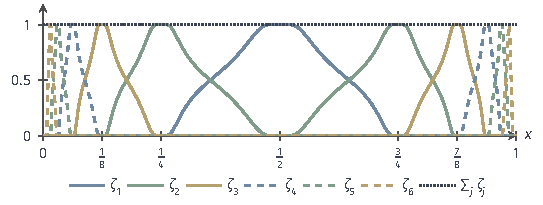
\includegraphics[width=92.0mm]{figures/02-abstract-mathematics/03-function-spaces/tikz/c4-partition-unity/figure.pdf}
  \caption{$\Omega=(0,1)$上的局部有限单位分解。记$s=\min(x,1-x)$为到边界的距离，$\zeta_j$支撑在$2^{-j-1}\le s\le2^{-j+1}$内，紧含于$(0,1)$；图中画出$\zeta_1,\ldots,\zeta_6$，每点至多两个权重非零，所有权重之和恒为$1$（点线）。越靠近边界，权重越密集，对应的磨光半径也要越小。}
  \label{fig:sob-partition-unity}
\end{figure}

\begin{theorem}[整域光滑逼近]
\label{thm:sob-meyers-serrin}
设$\Omega\subset\mathbb R^d$为任意开集，$k\ge0$，$1\le p<\infty$。则$C^\infty(\Omega)\cap W^{k,p}(\Omega)$在$W^{k,p}(\Omega)$中稠密。
\end{theorem}

\begin{proof}
固定$u\in W^{k,p}(\Omega)$与$\eta>0$。

第一步，分块。令$u_j=\zeta_ju$。由第~\ref{sec:sob-weak-derivative-def}节与光滑函数相乘的乘积法则（对高阶导数反复使用），$u_j\in W^{k,p}(\Omega)$，其各阶弱导数是$\zeta_j$的导数与$u$的弱导数的乘积之和，支撑在$V_j$内。由于$\zeta_j$紧支撑在$\Omega$内，把$u_j$在$\Omega$外补成零后属于$W^{k,p}(\mathbb R^d)$：对$\mathbb R^d$上的测试$\varphi$，用一个在$\operatorname{supp}\zeta_j$上为$1$、支撑在$\Omega$内的截断$\chi$，有$\int u_jD^\alpha\varphi=\int u_jD^\alpha(\chi\varphi)$，而$\chi\varphi$是$\Omega$上的测试。

第二步，逐块磨光并分配误差。对每个$j$，由定理~\ref{thm:sob-local-approximation}在$\mathbb R^d$上的结论，取$\varepsilon_j>0$足够小，使$v_j=u_j*\rho_{\varepsilon_j}$满足
\[
 \|v_j-u_j\|_{W^{k,p}(\mathbb R^d)}<\eta\,2^{-j},
\]
并且$\operatorname{supp}v_j\subset W_j:=G_{j+2}\setminus\overline{G_{j-2}}$。后一要求可以满足：$v_j$的支撑落在$\operatorname{supp}u_j$的$\varepsilon_j$邻域内，而$\overline{G_{j+1}}\subset G_{j+2}$、$\overline{G_{j-2}}\subset G_{j-1}$都是紧集含于开集，$V_j$与$W_j$的补集之间有正的间隔，取$\varepsilon_j$小于这个间隔即可。这里给第$j$块分配误差$\eta2^{-j}$，是为了让总和不超过$\eta$。

第三步，拼合。令$v=\sum_jv_j$。每点有邻域只与有限多个$W_j$相交，所以在这个邻域上$v$是有限个光滑函数之和，$v\in C^\infty(\Omega)$。同理$u=\sum_ju_j$在每个$G_m$上也只是有限和。于是在$G_m$上
\[
 \|v-u\|_{W^{k,p}(G_m)}\le\sum_j\|v_j-u_j\|_{W^{k,p}(\mathbb R^d)}<\sum_j\eta2^{-j}=\eta .
\]
令$m\to\infty$，由单调收敛定理（第~\ref{sec:measure-general-structure}节），$\|v-u\|_{W^{k,p}(\Omega)}\le\eta$。特别地$v\in W^{k,p}(\Omega)$。
\end{proof}

这个定理对任意开集成立，连边界的形状都不需要。但要读清它给出的是什么：逼近函数在$\Omega$\emph{内部}光滑，可能在边界附近剧烈振荡，并不是“光滑到边界”的函数，更不是紧支撑在$\Omega$内的测试函数。$C_c^\infty(\Omega)$在$W^{k,p}(\Omega)$中一般\emph{不}稠密。以$(0,1)$上的常数$1$为例：每个$\varphi\in C_c^\infty(0,1)$在端点附近为零，由式~\eqref{eq:sob-1d-sup-bound}（$p=2$，$L=1$），
\[
 1=|1-\varphi(0)|\le\|1-\varphi\|_{L^2}+\|(1-\varphi)'\|_{L^2}\le\sqrt2\,\|1-\varphi\|_{H^1},
\]
所以常数$1$到$C_c^\infty(0,1)$的$H^1$距离至少是$1/\sqrt2$。测试函数的闭包把“边界值为零”的信息保留了下来，这将在第~\ref{sec:sob-poincare}节定义$H_0^1$。

\paragraph{光滑到边界：从半空间反射开始}
许多论证需要更强的逼近：逼近函数在闭区域$\overline\Omega$上光滑，即是某个$C_c^\infty(\mathbb R^d)$函数在$\Omega$上的限制。思路是先把$u$延拓成全空间上的Sobolev函数，再在全空间磨光，最后限制回$\Omega$。延拓是关键，而延拓方式的好坏取决于边界。

最简单的区域是半空间$\mathbb R^d_+=\{x=(x',x_d):x_d>0\}$，这里$x'\in\mathbb R^{d-1}$。对光滑到边界的$u$，作偶反射
\[
 Eu(x',x_d)=u(x',|x_d|).
\]
它在$x_d=0$处连续，但沿$x_d$方向一般出现尖点。像$|x|$那样在两侧分别分部积分，边界面上的项因两侧的值相同而相消，所以$Eu$有弱导数：对$j<d$，$\partial_jEu(x',x_d)=(\partial_ju)(x',|x_d|)$；对$j=d$，$\partial_dEu(x',x_d)=\operatorname{sgn}(x_d)\,(\partial_du)(x',|x_d|)$。两侧对称，所以
\[
 \|Eu\|_{W^{1,p}(\mathbb R^d)}^p=2\,\|u\|_{W^{1,p}(\mathbb R^d_+)}^p .
\]
一般的$u\in W^{1,p}(\mathbb R^d_+)$可以先向区域内部平移一小段再磨光，得到光滑到边界的逼近，再由上式把延拓推广过去；这一细节属于补充，这里不展开。

与偶反射对照，零延拓（在$x_d<0$处令$u=0$）通常不行：若$u$在边界面上的值不为零，零延拓在边界面上产生跳跃，按阶跃函数的计算，它的$x_d$方向广义导数含有一个集中在边界面上的项，不是局部可积函数。图~\ref{fig:sob-reflection}在一维比较了两种延拓。只有当$u$的边界值为零时（确切含义见第~\ref{sec:sob-trace}节），零延拓才保持在$W^{1,p}$中。高阶空间中偶反射也不够，因为$x_d$方向的导数在反射后改变符号而跳跃；可以改用$Eu(x',x_d)=-3u(x',-x_d)+4u(x',-x_d/2)$（$x_d<0$），容易核对它在边界面上与$u$的值和一阶法向导数都相接。

\begin{figure}[!htb]
  \centering
  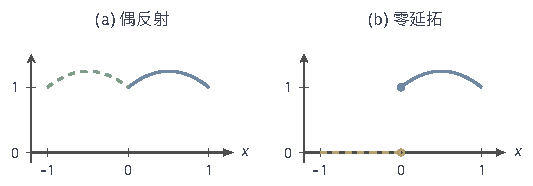
\includegraphics[width=90.2mm]{figures/02-abstract-mathematics/03-function-spaces/tikz/c4-reflection/figure.pdf}
  \caption{半区间上的两种延拓，$u(x)=1+x-x^2$（$0\le x\le1$），$u(0)=1$。(a)~偶反射$Eu(x)=u(|x|)$（虚线为延拓部分）：在原点连续而有尖点，弱导数$\operatorname{sgn}(x)u'(|x|)$局部可积，延拓保持在$W^{1,p}$中。(b)~零延拓：在原点跳跃$u(0)=1$，广义导数含$\delta_0$项，延拓不在$W^{1,p}$中。}
  \label{fig:sob-reflection}
\end{figure}

\paragraph{Lipschitz区域与延拓}
一般区域的边界可以弯曲，但只要它在局部可以拉直成半空间，就能沿用反射。

\begin{definition}[Lipschitz区域]
\label{def:sob-lipschitz-domain}
称有界开集$\Omega\subset\mathbb R^d$为\term{Lipschitz区域}（Lipschitz domain），若对每个$x_0\in\partial\Omega$，存在$r>0$、一个以$x_0$为原点的旋转后的坐标系$(x',x_d)$和Lipschitz函数$\gamma:\mathbb R^{d-1}\to\mathbb R$，使
\[
 \Omega\cap B(x_0,r)=\{x\in B(x_0,r):x_d>\gamma(x')\}.
\]
\end{definition}

也就是说，在每个边界点附近，区域位于一个Lipschitz函数图像的上方，边界就是这个图像。球、立方体、凸多面体都是Lipschitz区域：立方体的棱角处边界不光滑，但仍是局部的Lipschitz图像。挖去一条线段的圆盘（割缝圆盘）不是：割缝两侧都是区域，区域不能只位于割缝的一侧。尖角向内收缩得比任何Lipschitz图像都快的区域也不是。

\begin{theorem}[Lipschitz区域上的延拓]
\label{thm:sob-extension}
设$\Omega$为有界Lipschitz区域，$1\le p<\infty$。存在有界线性算子$E:W^{1,p}(\Omega)\to W^{1,p}(\mathbb R^d)$，使$Eu=u$在$\Omega$上几乎处处成立，并且所有$Eu$都支撑在同一个有界集合内。
\end{theorem}

证明思路如下，细节属于补充阅读。边界是紧集，可以用有限个满足定义的球$B(x_i,r_i)$覆盖，再加上一个紧含于$\Omega$的开集覆盖内部；取从属于这有限个开集的单位分解，把$u$分成有限块。内部那块直接零延拓，它在边界附近本来就是零。每个边界块用变换$(x',x_d)\mapsto(x',x_d-\gamma(x'))$拉直：这个变换和它的逆都是Lipschitz的，可以证明它们把$W^{1,p}$函数变成$W^{1,p}$函数，范数只差一个由$\gamma$的Lipschitz常数决定的倍数。拉直后在半空间上作偶反射，再变换回去。有限多块的延拓相加，得到$Eu$。这里每一步都需要边界是局部的Lipschitz图像，割缝圆盘之所以失败，正是因为割缝两侧都有区域，无法只向一侧反射。

\begin{theorem}[光滑到边界的逼近]
\label{thm:sob-smooth-up-to-boundary}
设$\Omega$为有界Lipschitz区域，$1\le p<\infty$。则$C_c^\infty(\mathbb R^d)$中函数在$\Omega$上的限制在$W^{1,p}(\Omega)$中稠密。
\end{theorem}

\begin{proof}
对$u\in W^{1,p}(\Omega)$，由定理~\ref{thm:sob-extension}得到紧支撑的$Eu\in W^{1,p}(\mathbb R^d)$。由定理~\ref{thm:sob-local-approximation}，$Eu*\rho_\varepsilon\to Eu$在$W^{1,p}(\mathbb R^d)$中成立，而$Eu*\rho_\varepsilon\in C_c^\infty(\mathbb R^d)$。限制到$\Omega$上，范数只会变小，所以$\|(Eu*\rho_\varepsilon)|_\Omega-u\|_{W^{1,p}(\Omega)}\le\|Eu*\rho_\varepsilon-Eu\|_{W^{1,p}(\mathbb R^d)}\to0$。
\end{proof}

记这类限制函数的全体为$C^\infty(\overline\Omega)$。与定理~\ref{thm:sob-meyers-serrin}比较，它多了边界正则性的条件，换来了在闭区域上光滑、各阶导数连续到边界的逼近函数。下一节的边界迹就要用到这一点：对光滑到边界的函数，边界值有经典含义，再用逼近推广到整个Sobolev空间。
